\documentclass[a4paper,11pt,twoside]{memoir}

% Castellano
\usepackage[spanish,es-tabla]{babel}
\selectlanguage{spanish}
\usepackage[utf8]{inputenc}
\usepackage{placeins}
\usepackage{eurosym}
\usepackage{float}

%ANDRES
\usepackage{amsmath, mathtools}

\RequirePackage{booktabs}
\RequirePackage[table]{xcolor}
\RequirePackage{xtab}
\RequirePackage{multirow}


% Links
\usepackage[colorlinks]{hyperref}
\hypersetup{
	allcolors = {red}
}

% Ecuaciones
\usepackage{amsmath}

% Rutas de fichero / paquete
\newcommand{\ruta}[1]{{\sffamily #1}}

% Párrafos
\nonzeroparskip


% Imagenes
\usepackage{graphicx}
\newcommand{\imagen}[2]{
	\begin{figure}[!h]
		\centering
		\includegraphics[width=0.9\textwidth]{#1}
		\caption{#2}\label{fig:#1}
	\end{figure}
	\FloatBarrier
}

\newcommand{\imagenDos}[3]{
	\begin{figure}[!h]
		\centering
		\includegraphics[width=#3\textwidth]{#1}
		\caption{#2}\label{fig:#1}
	\end{figure}
	\FloatBarrier
}

\newcommand{\imagenflotante}[2]{
	\begin{figure}%[!h]
		\centering
		\includegraphics[width=0.9\textwidth]{#1}
		\caption{#2}\label{fig:#1}
	\end{figure}
}


%%%%%%%%%%%   COMANDOS ANDRES  $$$$$$$$$$$$$$$$$$$$$$

\newcommand{\imagenCustom}[4]{
	\begin{figure}[!h]
		\centering
		\includegraphics[width=#4\textwidth]{#1}
		\caption{#2}
		\label{fig:#3}
	\end{figure}
	\FloatBarrier
}

\newcommand{\imagenCustomSinRef}[5]{
	\begin{figure}[!h]
		\centering
		\includegraphics[width=#4\textwidth]{#1}
		\caption[#5]{#2}
		\label{fig:#3}
	\end{figure}
	\FloatBarrier
}
%%%%%%%%%%%%%%%%%%%%%%%%%$$$$$$$$$$$$$$$$$$$$$$$$$$$$$



% El comando \figura nos permite insertar figuras comodamente, y utilizando
% siempre el mismo formato. Los parametros son:
% 1 -> Porcentaje del ancho de página que ocupará la figura (de 0 a 1)
% 2 --> Fichero de la imagen
% 3 --> Texto a pie de imagen
% 4 --> Etiqueta (label) para referencias
% 5 --> Opciones que queramos pasarle al \includegraphics
% 6 --> Opciones de posicionamiento a pasarle a \begin{figure}
\newcommand{\figuraConPosicion}[6]{%
  \setlength{\anchoFloat}{#1\textwidth}%
  \addtolength{\anchoFloat}{-4\fboxsep}%
  \setlength{\anchoFigura}{\anchoFloat}%
  \begin{figure}[#6]
    \begin{center}%
      \Ovalbox{%
        \begin{minipage}{\anchoFloat}%
          \begin{center}%
            \includegraphics[width=\anchoFigura,#5]{#2}%
            \caption{#3}%
            \label{#4}%
          \end{center}%
        \end{minipage}
      }%
    \end{center}%
  \end{figure}%
}

%
% Comando para incluir imágenes en formato apaisado (sin marco).
\newcommand{\figuraApaisadaSinMarco}[5]{%
  \begin{figure}%
    \begin{center}%
    \includegraphics[angle=90,height=#1\textheight,#5]{#2}%
    \caption{#3}%
    \label{#4}%
    \end{center}%
  \end{figure}%
}
% Para las tablas
\newcommand{\otoprule}{\midrule [\heavyrulewidth]}
%
% Nuevo comando para tablas pequeñas (menos de una página).
\newcommand{\tablaSmall}[5]{%
 \begin{table}[H]
  \begin{center}
   \rowcolors {2}{gray!35}{}
   \begin{tabular}{#2}
    \toprule
    #4
    \otoprule
    #5
    \bottomrule
   \end{tabular}
   \caption{#1}
   \label{tabla:#3}
  \end{center}
 \end{table}
}

%
% Nuevo comando para tablas pequeñas (menos de una página).
\newcommand{\tablaSmallSinColores}[5]{%
 \begin{table}[H]
  \begin{center}
   \begin{tabular}{#2}
    \toprule
    #4
    \otoprule
    #5
    \bottomrule
   \end{tabular}
   \caption{#1}
   \label{tabla:#3}
  \end{center}
 \end{table}
}

\newcommand{\tablaApaisadaSmall}[5]{%
\begin{landscape}
  \begin{table}
   \begin{center}
    \rowcolors {2}{gray!35}{}
    \begin{tabular}{#2}
     \toprule
     #4
     \otoprule
     #5
     \bottomrule
    \end{tabular}
    \caption{#1}
    \label{tabla:#3}
   \end{center}
  \end{table}
\end{landscape}
}

%
% Nuevo comando para tablas grandes con cabecera y filas alternas coloreadas en gris.
\newcommand{\tabla}[6]{%
  \begin{center}
    \tablefirsthead{
      \toprule
      #5
      \otoprule
    }
    \tablehead{
      \multicolumn{#3}{l}{\small\sl continúa desde la página anterior}\\
      \toprule
      #5
      \otoprule
    }
    \tabletail{
      \hline
      \multicolumn{#3}{r}{\small\sl continúa en la página siguiente}\\
    }
    \tablelasttail{
      \hline
    }
    \bottomcaption{#1}
    \rowcolors {2}{gray!35}{}
    \begin{xtabular}{#2}
      #6
      \bottomrule
    \end{xtabular}
    \label{tabla:#4}
  \end{center}
}

%
% Nuevo comando para tablas grandes con cabecera.
\newcommand{\tablaSinColores}[6]{%
  \begin{center}
    \tablefirsthead{
      \toprule
      #5
      \otoprule
    }
    \tablehead{
      \multicolumn{#3}{l}{\small\sl continúa desde la página anterior}\\
      \toprule
      #5
      \otoprule
    }
    \tabletail{
      \hline
      \multicolumn{#3}{r}{\small\sl continúa en la página siguiente}\\
    }
    \tablelasttail{
      \hline
    }
    \bottomcaption{#1}
    \begin{xtabular}{#2}
      #6
      \bottomrule
    \end{xtabular}
    \label{tabla:#4}
  \end{center}
}

%
% Nuevo comando para tablas grandes sin cabecera.
\newcommand{\tablaSinCabecera}[5]{%
  \begin{center}
    \tablefirsthead{
      \toprule
    }
    \tablehead{
      \multicolumn{#3}{l}{\small\sl continúa desde la página anterior}\\
      \hline
    }
    \tabletail{
      \hline
      \multicolumn{#3}{r}{\small\sl continúa en la página siguiente}\\
    }
    \tablelasttail{
      \hline
    }
    \bottomcaption{#1}
  \begin{xtabular}{#2}
    #5
   \bottomrule
  \end{xtabular}
  \label{tabla:#4}
  \end{center}
}



\definecolor{cgoLight}{HTML}{EEEEEE}
\definecolor{cgoExtralight}{HTML}{FFFFFF}

%
% Nuevo comando para tablas grandes sin cabecera.
\newcommand{\tablaSinCabeceraConBandas}[5]{%
  \begin{center}
    \tablefirsthead{
      \toprule
    }
    \tablehead{
      \multicolumn{#3}{l}{\small\sl continúa desde la página anterior}\\
      \hline
    }
    \tabletail{
      \hline
      \multicolumn{#3}{r}{\small\sl continúa en la página siguiente}\\
    }
    \tablelasttail{
      \hline
    }
    \bottomcaption{#1}
    \rowcolors[]{1}{cgoExtralight}{cgoLight}

  \begin{xtabular}{#2}
    #5
   \bottomrule
  \end{xtabular}
  \label{tabla:#4}
  \end{center}
}






\graphicspath{ {./img/} }

% Capítulos
\chapterstyle{bianchi}
\newcommand{\capitulo}[2]{
	\setcounter{chapter}{#1}
	\setcounter{section}{0}
	\chapter*{#2}
	\addcontentsline{toc}{chapter}{#2}
	\markboth{#2}{#2}
}

% Apéndices
\renewcommand{\appendixname}{Apéndice}
\renewcommand*\cftappendixname{\appendixname}

\newcommand{\apendice}[1]{
	%\renewcommand{\thechapter}{A}
	\chapter{#1}
}

\renewcommand*\cftappendixname{\appendixname\ }

% Formato de portada
\makeatletter
\usepackage{xcolor}
\newcommand{\tutor}[1]{\def\@tutor{#1}}
\newcommand{\course}[1]{\def\@course{#1}}
\definecolor{cpardoBox}{HTML}{E6E6FF}
\def\maketitle{
  \null
  \thispagestyle{empty}
  % Cabecera ----------------
\noindent\includegraphics[width=\textwidth]{cabecera}\vspace{1cm}%
  \vfill
  % Título proyecto y escudo informática ----------------
  \colorbox{cpardoBox}{%
    \begin{minipage}{.8\textwidth}
      \vspace{.5cm}\Large
      \begin{center}
      \textbf{TFG del Grado en Ingeniería Informática}\vspace{.6cm}\\
      \textbf{\LARGE\@title{}}
      \end{center}
      \vspace{.2cm}
    \end{minipage}

  }%
  \hfill\begin{minipage}{.20\textwidth}
    
\includegraphics[width=\textwidth]{escudoInfor}
  \end{minipage}
  \vfill
  % Datos de alumno, curso y tutores ------------------
  \begin{center}%
  {%
    \noindent\LARGE
    Presentado por \@author{}\\ 
    en Universidad de Burgos --- 3 de julio de 2017\\
    Tutor: \@tutor{}\\
  }%
  \end{center}%
  \null
  \cleardoublepage
  }
\makeatother


% Datos de portada
\title{Análisis paleontológico de piezas dentales 2.0 \\Documentación Técnica}
\author{Andrés Miguel Terán}
\tutor{Dr. José Francisco Díez Pastor\\Tutor: Dr. Raúl Marticorena Sánchez}
\date{\today}

\begin{document}

\maketitle



\cleardoublepage

%%%%%%%%%%%%%%%%%%%%%%%%%%%%%%%%%%%%%%%%%%%%%%%%%%%%%%%%%%%%%%%%%%%%%%%%%%%%%%%%%%%%%%%%



\frontmatter


\clearpage

% Indices
\tableofcontents

\clearpage

\listoffigures

\clearpage

\listoftables

\clearpage

\mainmatter

\appendix

\apendice{Plan de Proyecto Software}

\section{Introducción}
En este apartado se expondrá la metodología y planificación del proyecto adoptada así como las herramientas utilizadas.

La metodología de desarrollo ágil utilizada ha sido \emph{SCRUM}. Cada semana o semana y media se realizaba una reunión con los tutores para definir y organizar las tareas a realizar durante el siguiente \textit{sprint}.

Como sistema de control de versiones se ha usado \emph{git} mediante un repositorio online en GitHub y su aplicación \emph{GitHub Desktop} para Windows y la herramienta de git que ofrece \emph{Eclipse} para entornos Linux.

Se ha utilizado también \emph{ZenHub}, un plugin para navegadores que se integra en GitHub y permite la gestión del proyecto incluyendo además la posibilidad de ver distintos gráficos para comprobar como van los avances. Ha sido muy útil para organizar las tareas y poder seguir la metodología \emph{SCRUM}.

\newpage

\section{Planificación temporal}
A continuación se muestra el avance a lo largo de las iteraciones que forman el proyecto:

\subsection{Sprint 1: }
27/01/2017 - 03/02/2017 (figura \ref{fig:img/BurndownCharts/chart1})

\imagen{img/BurndownCharts/chart1}{Burndown Chart Sprint 1}

\begin{itemize}
    \item Instalación y preparación de maquinas virtuales.
    \item Recompilar y probar la aplicación de \textit{stitching} que hay hecha en un sistema Linux de 64 bits.
    \item Adaptar la aplicación Java para el \textit{stitching} en Linux de 64 bits.
    \item Recompilar \textit{Stitching.exe} para sistemas Windows de 32 bits.
\end{itemize}

Este \textit{sprint} me ha servido para familiarizarme con el proyecto, preparar su entorno y empezar a trabajar con la aplicación de \textit{stitching} a revisar, centrándome en su recompilación para que pueda ser ejecutado en sistemas de distintas arquitecturas y distintos sistemas operativos. 

\newpage

\subsection{Sprint 2:}
04/02/2017 - 15/02/2017 (figura \ref{fig:img/BurndownCharts/chart2})

\imagen{img/BurndownCharts/chart2}{Burndown Chart Sprint 2}

\begin{itemize}
    \item Probar \textit{stitching} Linux en equipos Linux de 32 bits.
    \item Recompilar \textit{stitching} para Linux 32 bits.
    \item Adaptar la aplicación para que seleccione un \textit{stitching} u otro dependiendo del sistema operativo y la arquitectura.
    \item Comenzar la memoria.
\end{itemize}

En este \textit{sprint} se ha realizado la recompilación del \textit{stitching} para distribuciones Linux de 32 bits. No ha sido posible utilizar esta versión en sistemas Linux de 64 bits, por lo que se ha decidido que el \textit{stitching} para 64 bits forme parte de la aplicación también. 

\newpage

\subsection{Sprint 3:} 
17/02/2017 - 01/03/2017 (figura \ref{fig:img/BurndownCharts/chart3})

\imagen{img/BurndownCharts/chart3}{Burndown Chart Sprint 3}

\begin{itemize}
    \item Comprobar el uso de carpetas temporales y permisos con Java.
    \item Crear una opción de seleccionar un carpeta para archivos temporales.
    \item Adaptar el código Java para extraer los fragmentos de las imágenes de rutas sin espacios en blanco.
    \item Adaptar el código Java para comprobar que los fragmentos no están en una ruta con espacios en blanco.
    \item Continuar la documentación.
\end{itemize}

La aplicación de \textit{stitching} no funcionaba en determinadas ocasiones, se ha detectado que es debido a que la ruta de las imágenes contienen espacios en blanco. Para solucionarlo se ha decidido usar una carpeta temporal válida donde poder hacer el \textit{stitching} sin problemas. Esta carpeta es la carpeta temporal del sistema por defecto o una que elija el usuario.

\newpage

\subsection{Sprint 4:} 
26/02/2017 - 02/03/2017 (figura \ref{fig:img/BurndownCharts/chart4})

\imagen{img/BurndownCharts/chart4}{Burndown Chart Sprint 4}

\begin{itemize}
    \item Solucionar el error ejecución de \textit{stitching} desde el archivo ejecutable \textit{.jar}.
    \item Realizar un test unitario sobre la clase \textit{StitchingTemporaryUtil.java}.
    \item Utilizar distintos parámetros mediante \textit{interact} de los \textit{Jupyter notebooks} para comprobar la eficacia en la detección de bordes sobre las imágenes disponibles.
\end{itemize}

La aplicación Java, cuando se exportaba a un fichero \textit{jar}, no podía hacer uso de la aplicación de \textit{stitching} que tenía comprimida en dentro de la carpeta \textit{rsc}. Se ha adaptado el código para que la aplicación Java pueda descomprimirla y usarla. También se ha comenzado la búsqueda de filtros más adecuados para la detección de perikymata usando los \textit{Jupyter notebooks}.

Al finalizar este sprint se ha sacado una \textit{release} en su versión 1.1 porque el cliente necesita hacer uso de la aplicación ahora que ya tiene solucionado el error del \textit{stitching}.

\newpage

\subsection{Sprint 5:}
03/03/2017 - 03/03/2017 (figura \ref{fig:img/BurndownCharts/chart5})

\imagen{img/BurndownCharts/chart5}{Burndown Chart Sprint 5}

\begin{itemize}
    \item Estudiar el funcionamiento de la matriz Hessiana y el filtro Frangi para su aplicación a la detección de bordes.
    \item Probar si directamente \textit{ImageJ} para Java resulta más sencillo de aplicar que \textit{Scikit-Image} para Python.
    \item Comenzar a evaluar como de buena es una propuesta filtrada.
\end{itemize}

\textit{ImageJ} es una librería usada para el procesamiento de imagen que pensábamos emplear, aunque finalmente se va a utilizar \textit{Scikit-Image} para Python porque es más sencillo de usar y aprender. Además, permite ver los resultados de manera rápida a través de los \textit{notebooks}. Posteriormente, todo el código Python habrá que buscar alguna manera de exportarlo a algún ejecutable que pueda ser llamado desde Java.

El filtro de Frangi es con el que he comenzado y una posible forma de evaluar su eficacia es mediante la \textit{distancia de Levenshtein}\footnote{Se obtuvo una implementación de aquí: \url{https://es.wikipedia.org/wiki/Distancia_de_Levenshtein}.}.

\newpage

\subsection{Sprint 6:}
11/03/2017 - 17/03/2017 (figura \ref{fig:img/BurndownCharts/chart6})

\imagen{img/BurndownCharts/chart6}{Burndown Chart Sprint 6}

\begin{itemize}
    \item Comparar máscara y nuevo método con los datos del CSV.
    \item Realizar evaluación sobre imágenes filtradas (método antiguo Prewitt). Modificar el umbral para realizar las pruebas.
    \item Obtener recursivamente imágenes para pruebas.
    \item Crear módulo en Python para la nueva técnica de filtrado.
    \item Investigar las mejores opciones para exportar la aplicación de Python a ejecutables.
    \item Crear test con imágenes de distintos tamaños.
    \item Probar paso a paso ejecución del filtro nuevo con una imagen grande.
\end{itemize}

En este \textit{sprint} se ha creado una máscara de usuario para comparar con los resultados del filtro de Frangi sobre distintas imágenes. 

Los resultados eran prometedores hasta que se han realizado pruebas con una imagen de un diente, en tamaño más grande, y los resultado son notablemente peor que sobre un trozo pequeño de imagen.

Se ha buscado también, crear una función que permita optimizar los parámetros para obtener los mejores resultados sobre la \textit{distancia de Levenshtein}.

\newpage

\subsection{Sprint 7:}
18/03/2017 - 24/03/2017 (figura \ref{fig:img/BurndownCharts/chart7})

\imagen{img/BurndownCharts/chart7}{Burndown Chart Sprint 7}

\begin{itemize}
    \item Incluir y ver que resultados da el filtro Prewitt con el nuevo método.
    \item Crear un notebook paso a paso para encontrar errores e incluir mejoras.
    \item Preparar un script para utilizar PyInstaler (instalar todo primero).
\end{itemize}

En esta iteración se han realizado más pruebas, añadiendo al método creado el filtro Prewitt, para ver como mejora o empeora el resultado sobre una imagen de diente a tamaño completo. También se ha decidido utilizar PyInstaller para exportar código Python a un ejecutable porque es el único de varias alternativas que lo crea con todas las dependencias comprimidas.

\newpage

\subsection{Sprint 8:}
25/03/2017 - 31/03/2017 (figura \ref{fig:img/BurndownCharts/chart8})

\imagen{img/BurndownCharts/chart8}{Burndown Chart Sprint 8}

\begin{itemize}
    \item Probar si PyInstaller realiza correctamente las importaciones de los módulos en Python.
    \item Probar la binarización de imagen antes de aplicar Frangi.
    \item Probar la utilización de umbrales adaptativos para la imagen.
    \item Incluir en la función a optimizar el tratamiento de excepciones.
    \item Crear una máscara del diente 2.
\end{itemize}

En el pequeño script de prueba realizado con PyInstaler no ha habido problemas y funciona correctamente, pero al exportar todo el código Python, la aplicación no consigue funcionar. Queda pendiente para la próxima iteración.

Los umbrales adaptativos han funcionado correctamente y se incluirán en la versión final del procesado de imagen. Para próximos sprints se va a probar con la imagen del diente 2 porque la del diente 1 no es muy apta para los procesados, también se tiene incertidumbre porque solo hay dos imágenes de dientes y se desconoce cual es el caso normal que se encuentran en el Laboratorio de la Evolución Humana, que sea una imagen donde no se aprecian las perikymata o que se vean de forma aceptable.

\newpage

\subsection{Sprint 9:}
01/04/2017 - 08/04/2017 (figura \ref{fig:img/BurndownCharts/chart9})

\imagen{img/BurndownCharts/chart9}{Burndown Chart Sprint 9}

\begin{itemize}
    \item Probar el \textit{.exe} conseguido con PyInstaller con rutas absolutas.
    \item Probar el \textit{.exe} conseguido con PyInstaller con imagen hardcodeada.
    \item Probar el procesado con el diente 2.
    \item Continuar la documentación.
\end{itemize}
Se han probado distintas opciones sobre el ejecutable en Windows que crea PyInstaler con el código en Python y se ha descubierto la necesidad de incluir unos archivos llamados \textit{hooks-files} para importar módulos ocultos de Python, por lo que la exportación se realiza satisfactoriamente.

Con la imagen del diente 2 el procesado gana eficacia. Descartamos por tanto, basar el código en conseguir que sea eficaz en la imagen del diente 1 ya que se intuye que el proceso falla más porque en la imagen no se ven las perikymata, que porque el proceso esté mal desarrollado.

El proyecto sobre dietas \cite{dietasIsma} ya tiene implementado funciones para trabajar con líneas, se probarán en el próximo \textit{sprint}.

\newpage

\subsection{Sprint 10:}
10/04/2017 - 17/04/2017 (figura \ref{fig:img/BurndownCharts/chart10})
\imagen{img/BurndownCharts/chart10}{Burndown Chart Sprint 10}
\begin{itemize}
    \item Estudiar el \textit{notebook} proporcionado sobre extracción de líneas.
    \item Revisar el algoritmo \textit{k\_components}  para adaptar o reutilizar.
    \item Realizar pruebas incluyendo el filtrado por direcciones.
    \item Implementar una función para cargar recursivamente imágenes de una carpeta.
\end{itemize}

En este \textit{sprint} se ha revisado la clase de Python \textit{Procesado.py} del trabajo de dietas \cite{dietasIsma} porque incluye un algoritmo de detección y unión de líneas usando teoría de grafos. 

Finalmente no se han utilizado las funciones relacionadas con los grafos, sino que se ha modificado el uso de la función de la \textit{Transformada de Hough} para operar en ciertos ángulos detectando líneas satisfactoriamente.

Investigando se han encontrado otros filtros como Sobel \cite{wiki:Sobel} y Kirsch \cite{scholar:venmathi2016kirsch}, que se probarán más adelante, porque resaltan bordes en direcciones personalizadas.

\newpage

\subsection{Sprint 11:}
18/04/2017 - 21/04/2017 (figura \ref{fig:img/BurndownCharts/chart11})
\imagen{img/BurndownCharts/chart11}{Burndown Chart Sprint 11}
\begin{itemize}
    \item Probar el filtro Sobel sobre la imagen completa del diente.
    \item Implementar una función para usar el operador de Kirsch.
    \item Probar el operador de Kirsch con diferentes filtrados.
    \item Añadir el filtrado por direcciones.
    \item Aplicar la operación de convolución manualmente con varios operadores. 
\end{itemize}

Los resultados con el operador de Kirsch, basado en este artículo \cite{scholar:venmathi2016kirsch}, son los más prometedores porque las perikymata no están siempre en la misma dirección y Kirsch permite elegir la orientación. 

Sobel \cite{wiki:Sobel} queda descartado por ser demasiado simple (solo opera en los ejes \textit{x} e \textit{y}).

\newpage

\subsection{Sprint 12:}
22/04/2017 - 28/04/2017 (figura \ref{fig:img/BurndownCharts/chart12})
\imagen{img/BurndownCharts/chart12}{Burndown Chart Sprint 12}
\begin{itemize}
    \item Probar el operador de Kirsch sobre el diente 1.
    \item Crear una función en Python que aplique el nuevo procesado de imagen basado en Kirsch. 
\end{itemize}

Al probar Kirsch sobre el diente 1, se detectan mejor algunas perikymata pero queda confirmado que la imagen del diente 1 no es adecuada para procesar, porque no se aprecian bien las perikymata.

En la reunión se ha hablado de simplificar la vista de conteo de perikymata y así ahorrar trabajo al usuario en la aplicación Java.

\newpage

\subsection{Sprint 13:}
29/04/2017 - 05/05/2017 (figura \ref{fig:img/BurndownCharts/chart13})
\imagen{img/BurndownCharts/chart13}{Burndown Chart Sprint 13}
\begin{itemize}
    \item Crear una función para rotar la imagen los grados que indique el usuario.
    \item Modificar la aplicación Java para recortar la imagen del diente.
    \item Ajustar la aplicación Java para incluir un \textit{BorderPane} con las nuevas funcionalidades.
    \item Ajustar el proceso de rotación para que la imagen se vea rotada.
\end{itemize}

En este \textit{sprint} se ha creado una nueva vista para rotar la imagen y que el usuario deje las perikymata de manera vertical para poder aplicar el filtro Kirsch y que las detecte correctamente.

\newpage

\subsection{Sprint 14:}
06/05/2017 - 11/05/2017 (figura \ref{fig:img/BurndownCharts/chart14})
\imagen{img/BurndownCharts/chart14}{Burndown Chart Sprint 14}
\begin{itemize}
    \item Estudiar la unión de la aplicación Java con la aplicación Python vía sockets.
    \item Crear un botón para restablecer la vista de una imagen recortada.
    \item Pasar la funcionalidad de medida de la escala desde la vista de conteo de perikymata a la vista de rotación de la imagen.
    \item Poner un fondo negro para el recortado de la imagen.
    \item Poner una imagen al botón de recortado.
    \item Limitar la rotación que se puede aplicar.
\end{itemize}

En esta iteración se ha mejorado la vista y la funcionalidad de rotación y recorte de la imagen.

\newpage
\subsection{Sprint 15:}
12/05/2017 - 17/05/2017 (figura \ref{fig:img/BurndownCharts/chart15})
\imagen{img/BurndownCharts/chart15}{Burndown Chart Sprint 15}
\begin{itemize}
    \item Incluir la creación de una carpeta \textit{Crop\_Image} para guardar la imagen recortada.
    \item Crear un prototipo de conexión Java-Python a través de sockets.
    \item Definir un protocolo de comunicación entre Java y Python.
    \item Implementar una función de \textit{handshake} entre Java y Python.
    \item Estudiar documento de reconstrucción de la corona del diente.
    \item Limpiar la vista de conteo de perikymata.
    \item Incluir migas de pan a lo largo de la aplicación.
\end{itemize}

Se ha terminado la funcionalidad de rotación y recortado de la imagen y se ha creado un prototipo de conexión por sockets en Python y Java donde Java es el servidor y Python el cliente. Se ha hablado en la que reunión que, para la siguiente iteración, queda pendiente cambiarlo para que el servidor sea Python.

Se han incluido las migas de pan en la aplicación para que el usuario sepa en que etapa está y para que sea más fácil moverse por la aplicación.

La reconstrucción de la corona permitirá calcular mejor las perikymata, se prevé una reunión con el personal del Laboratorio de la Evolución Humana para que nos expliquen el proceso de reconstrucción y dependiendo de su complejidad incluirlo en este proyecto o no.

\newpage

\subsection{Sprint 16:}
18/05/2017 - 29/05/2017 (figura \ref{fig:img/BurndownCharts/chart16})
\imagen{img/BurndownCharts/chart16}{Burndown Chart Sprint 16}
\begin{itemize}
    \item Implementar una función en Java para detectar píxeles rojos.
    \item Cambiar el servidor y cliente en Java y Python.
    \item Preparar el servidor en Python para la conexión con Java.
    \item Prepara la aplicación Java para la conexión con el servidor de Python.
    \item Arreglar el funcionamiento de las migas de pan.
    \item Arreglar el error detectado en la etapa de selección de imágenes.
    \item Aumentar la fuente y poner en negrita las migas de pan dependiendo donde nos encontremos.
\end{itemize}

En este sprint se han solucionado errores con las migas de pan y se ha localizado el origen y solucionado el error reportado que sucedía a veces al abrir la aplicación; en la carga inicial de imágenes, carga todos los elementos de la carpeta sean o no imágenes, lo cual da error al hacer el \textit{stitching}.

Se han modificado la aplicaciones de Java y Python y ya se comunican correctamente a través de sockets.

La detección de píxeles rojos se hace usando el modelo RGB \cite{wiki:RGB} y en la reunión se ha hablado de usar el modelo HSI \cite{wiki:spaceHSV_HSI_HSL} que permite ser más preciso en cuando al rojo.

\newpage

\subsection{Sprint 17:}
30/05/2017 - 06/06/2017 (figura \ref{fig:img/BurndownCharts/chart17})
\imagen{img/BurndownCharts/chart17}{Burndown Chart Sprint 17}
\begin{itemize}
    \item Incluir opciones avanzadas en la aplicación Java para aplicar filtros. 
    \item Redefinir el protocolo de comunicación en la parte del servidor Python.
    \item Utilizar el color HSI para extraer el color rojo de los píxeles, en vez de usar el RGB.
    \item Modificar procesado para guardar la imagen original con líneas detectadas superpuestas.
    \item Modificar la interfaz Java para alternar la imagen filtrada y la imagen filtrada con líneas superpuestas.
    \item Eliminar los falsos positivos al detectar perikymata.
    \item Separarlas coordenadas en la exportación de datos a \textit{csv}.
    \item Añadir el icono de zoom e icono de dibuja línea en la interfaz de conteo de perikymata.
    \item Escribir la introducción y objetivos de la memoria.
\end{itemize}

En este \textit{sprint} se han mejorado aspectos generales de la aplicación y del guardado de las imágenes filtradas. Además, se ha continuado con la memoria.

Finalmente se ha usado el espacio de color HSV\footnote{Llamado HSB en Java.} que sigue permitiéndonos conocer el matiz del color.

También se han encontrado errores en la interfaz de la aplicación al pasar a pantallas de tamaño 1366x768. Este error es debido a que el desarrollo de la aplicación ha sido en una pantalla de tamaño 1920x1080.

\subsection{Sprint 18:}
07/06/2017 - 15/06/2017
\imagen{img/BurndownCharts/chart18}{Burndown Chart Sprint 18}

\begin{itemize}
    \item Revisar la introducción y objetivos.
    \item Arreglar el redimensionado de la aplicación.
    \item Arreglar la petición de opciones avanzadas en el servidor Python.
    \item Documentar los conceptos teóricos.
    \item Implementar el correcto cerrado del servidor desde Java.
\end{itemize}

En esta iteración se han solucionado errores con las vistas de la aplicación y con la petición de filtrado avanzado.

Para el próximo \textit{sprint} se adecuará la aplicación para su funcionamiento en entornos Linux y se lanzará una pre-release.

\newpage

\subsection{Sprint 19:}
16/06/2017 - 22/06/2017 (figura \ref{fig:img/BurndownCharts/chart19})
\imagen{img/BurndownCharts/chart19}{Burndown Chart Sprint 19}
\begin{itemize}
    \item Volver a buscar formas de exportar el servidor de Python.
    \item Documentar Técnicas y Herramientas.
    \item Revisar el \textit{combobox} de selección de kernel en opciones avanzadas de filtrado.
    \item Mejorar la eficiencia en el guardado de las imágenes filtradas.
    \item Crear el manual de instalación y lanzar una release prototipo.
    \item Realizar arreglos en la aplicación para poder instalarla adecuadamente.
    \item Corregir las vistas para entornos Linux.
    \item Corregir el cargado de imágenes en Linux.
\end{itemize}

Este \textit{sprint} se ha caracterizado por preparar la aplicación para su instalación, probarla y adaptarla para entornos Linux.

Se han encontrado problemas a la hora de ver las vistas adecuadamente usando Ubuntu y la aplicación a veces se vuelve inestable, pero es usable.

Para la última iteración se terminará la memoria, se organizarán las pruebas realizadas en los \textit{Jupyter notebooks} y se finalizará el desarrollo de la aplicación.

\subsection{Sprint 20:}
23/06/2017 - 02/07/2017 (figura \ref{fig:img/BurndownCharts/chart20})
\imagen{img/BurndownCharts/chart20}{Burndow Chart Sprint 20}
Este último \textit{sprint} pone fin al proyecto, las tareas más relevantes han sido:
\begin{itemize}
    \item Finalizar toda la documentación del proyecto.
    \item Dar los últimos retoques a la aplicación.
    \item Organizar el contenido del proyecto.
    \item Solucionar los últimos errores encontrados.
\end{itemize}

\newpage
\section{Estudio de viabilidad}

En esta sección se hablará del apartado económico que concierne al desarrollo del proyecto. También trataremos el tema de su viabilidad legal.

\subsection{Viabilidad económica}

A continuación iremos nombrando y justificando todos los gastos que hubiera tenido el proyecto si no hubiera formado parte del plan de estudios del grado y se aplicase en un entorno real.

En la descripción del TFG se estima que el trabajo del alumno consiste en 300 horas, pero esto está alejado de la realidad por lo que usamos la herramienta ZenHub y a cada \textit{issue} le añadimos un valor numérico para estimar el tiempo. 

Cada unidad de tiempo añadida ha sido tomada con un valor real de 2 horas y tenemos 230 puntos por lo que la estimación de las horas invertidas quedaría en 460 horas.

En el proyecto anterior \cite{perikymataV1} se estimó la hora de trabajo del programador en 15\euro{} por lo que el coste del proyecto en mano de obra habría sido de:
\[15\text{\euro}/\text{h}\times 460\text{h}=6900\text{\euro} \]
Con este resultado tenemos que tener en cuenta el coste de la seguridad social que podemos obtener desde su página oficial\footnote{Página de la seguridad Social: \url{https://goo.gl/zRVeq9}.} y que nos dice que han de tenerse en cuenta los siguientes impuestos:
 \begin{itemize}
     \item Contingencias comunes: 23,60\%.
     \item Contrato duración determinada Tiempo parcial\footnote{Tomaremos que el proyecto tiene la duración de 5 meses a tiempo parcial.}: 6,70\%.
     \item Fondo de Garantía Salarial: 0,20\%.
     \item Formación Profesional: 0,60\%.
 \end{itemize}

Esto nos da un total de un 31,1\% en impuestos lo cual hace que el gasto destinado a la seguridad social sea de:
\[6900\text{\euro}\times 31,1\%=2139\text{\euro} \]

\newpage
También tenemos que valorar el coste de las herramientas hardware y software utilizadas en este proyecto de las cuales han tenido costes las siguientes:
\begin{itemize}
    \item Equipo de desarrollo (ordenador portátil): 730\euro{}.
    \item Periféricos usados (ratón, teclado y pantalla): 250\euro{}.
    \item Licencia Windows para usar en la máquina virtual: 121\euro{}\footnote{Se aplica el descuento a estudiantes. Fuente: \url{https://goo.gl/PwrrcP}.} .
\end{itemize}

El equipo de desarrollo y los periféricos hacen un total de 980\euro{} y según la agencia tributaria\footnote{Tablas de amortización 2017: \url{https://goo.gl/UTCRK9}.} los equipos para procesos de información tienen una vida útil de 8 años y este proyecto ha tenido una duración de 5 meses, 
lo cual nos deja unos costes de amortización de:

\[\frac{980\text{\euro}}{12 \text{ Meses}\times8 \text{ Años}} \times 5 \text{ Meses} =  51,04\text{\euro{}} \]

La licencia para la máquina virtual se ha usado durante los 5 meses de duración del proyecto pues continuamente se han tenido que probar los cambios realizados. Se estima su vida útil en 6 años por lo que sus costes de amortización serían los siguientes:

\[\frac{121\text{\euro}}{12 \text{ Meses}\times6 \text{ Años}} \times 5 \text{ Meses} =  8,40\text{\euro{}} \]

Esto nos deja un coste total en las herramientas utilizadas de 59.44\euro{}.

Con todos los costes mencionados, el desglose e importe final podemos observarlo en la tabla \ref{tabla:tablaCostes}


\tablaSmall{Costes del proyecto}{ll}{tablaCostes}{Costes & Importe\\}{
Personal & 6900\euro{}\\ 
Seguridad Social & 2139\euro{}\\ 
Herramientas & 59,44\euro{}\\ 
Total & 9098,44\euro{}\\ }

\subsection{Viabilidad legal}

La versión anterior del proyecto \cite{perikymataV1} usa una licencia GPL \cite{wiki:GPL} lo cual obliga a que esta también lo tenga y que la aplicación siga siendo software libre. Las nuevas partes añadidas como el servidor en Python y nuevos ficheros se les ha dotado también de una licencia GPL para mantener la coherencia de en toda la aplicación.

En este proyecto se ha prescindido de algunas librerías que usaba la versión anterior pero se han utilizado otras nuevas. También se han seguido usando las mismas imágenes e iconos que en la versión anterior además de añadir otros.

En la tabla \ref{tabla:licencias} podemos ver las licencias de las herramienta utilizadas.


\tablaSmall{Herramientas utilizadas y sus licencias}{l l}{licencias}{Herramienta & Licencia\\}{
Java JavaFX & Oracle Binary Code License\\
Python 3 & PSF License\\
Scikit-Image & BSD License\\
Numpy & BSD License \\
OpenCV & BSD License \\
Eclipse & Eclipse Public License\\
Visual Studio & Microsoft Software License\\
PyCharm & Apache 2.0 License \\
PyInstaller & GPL License\\
VirtualBox & GPL License\\ 
White Square icon & Public Domain \\
DesignContest Icons & CC Attribution 4.0\\
IconsMind Icons & LinkWare \\

}

\apendice{Especificación de Requisitos}

\section{Introducción}
En esta sección se hablará de los requisitos y casos de uso que han dado la hoja ruta a seguir para el desarrollo de la aplicación.
\section{Objetivos generales}
Los objetivos generales que persigue la aplicación, nos vienen dados desde el proyecto anterior \cite{perikymataV1}. Son los siguientes:
\begin{itemize}
    \item La aplicación debe poder unir las de imágenes de fragmentos del diente para ofrecer al usuario una imagen completa.
    \item Se debe poder aplicar un filtro o filtros para resaltar las perikymata de la imagen completa de la pieza dental. 
    \item Se debe poder delimitar la corona del diente en la imagen y dividirla en deciles sobre los que se dibujará una línea en la que se marcarán las perikymata detectadas.
    \item Todos los datos generados podrán ser guardados de forma persistente.
    \item Se deben corregir errores y mejorar cada una de las etapas mencionadas en la medida de lo posible, a fin de ser más eficaz en la detección de perikymata.
\end{itemize}

\pagebreak
\section{Catalogo de requisitos}
Los requisitos que debe satisfacer la aplicación son:
\begin{itemize}
        \item Se podrá introducir una imagen completa de una pieza dental. En caso de ser imágenes de fragmentos, se unirán formando la imagen completa.
        \item Se podrá preparar la imagen completa para su uso a lo largo de la aplicación.
        \item Se podrá aplicar un filtro a la imagen para resaltar las perikymata.
        \item Se detectarán y marcarán la perikymata en la imagen filtrada de manera automática, aunque el usuario podrá intervenir para corregir posibles errores.
        \item La aplicación guardará de manera automática las imágenes generadas y el usuario podrá exportar los datos generados.
        \item La aplicación deberá proporcionar las funcionalidades básicas de cualquier aplicación.
\end{itemize}

\section{Especificación de requisitos}

En este apartado se indicarán las especificación de los requisitos a cumplir.

\begin{itemize}
        \item RF-1: Introducir la imagen o imágenes de la pieza dental que usará la aplicación para conseguir una imagen completa.
            \begin{itemize}
                \item RF-1.1: Indicar un conjunto de imágenes y unirlas (\textit{stitching}).
                    \begin{itemize}
                        \item RF-1.1.1: Indicar un conjunto de imágenes válidas para unir que representan los fragmentos del diente.
                        \item RF-1.1.2: Unir la imágenes para obtener una imagen dental completa.
                    \end{itemize}
                \item RF-1.2: Indicar una imagen que represente la pieza dental completa.
            \end{itemize}              
                      
        \item RF-2: Preparar la imagen y datos para las etapas posteriores.
            \begin{itemize}
                \item RF-2.1: Rotar y recortar la imagen para orientar las perikymata de la forma más vertical posible y delimitar la zona de acción.
                \item RF-2.2: Indicar la escala a la que se encuentra la imagen de la pieza dental.      
            \end{itemize}
        
        \pagebreak        
        \item RF-3: Filtrar la imagen del diente y llevar a cabo la detección de perikymata.
            \begin{itemize}
                \item RF-3.1: Delimitar, de manera automática, los deciles de la corona dental.
                \item RF-3.2: Filtrar la imagen del diente gracias a un modo por defecto.
                \item RF-3.3: Filtrar la imagen del diente gracias a un modo avanzado con distintos parámetros de filtrado.
                \item RF-3.4: Dibujar una línea y marcar perikymata automáticamente.
                \begin{itemize}
                        \item RF-3.4.1: Dibujar una línea que atraviese las perikymata.
                        \item RF-3.4.2: Automarcar todas las perikymata que sean posibles. 
                \end{itemize}
                \item RF-3.5: Añadir o eliminar perikymata sobre la imagen filtrada.
            \end{itemize}        
        
        \item RF-4: Guardar todos los datos generados\footnote{Los cálculos realizados no se incluyen.}, incluidas las imágenes que intervienen en el proceso.
            \begin{itemize}
                \item RF-4.1: Guardar las imágenes que aporte el usuario y las que genere la aplicación en las carpetas del proyecto.
                \item RF-4.2: Almacenar, en formato \textit{csv}, los resultados generados sobre la distancia entre cada perikyma\footnote{\textit{Perikyma} es el singular de \textit{perikymata}.} y su localización en los deciles.
            \end{itemize}
            
        \item RF-5: Proporcionar acceso en todo momento a funcionalidades básicas de la aplicación.
            \begin{itemize}
                \item RF-5.1: Hacer uso de las \textit{migas de pan}.
                \begin{itemize}
                        \item RF-5.1.1: Ver la etapa actual de la aplicación en la que se encuentre el usuario.
                        \item RF-5.1.2: Retroceder a etapas anteriores de la aplicación.
                \end{itemize}
                \item RF-5.2: Abrir, cerrar y guardar el proyecto actual en cualquier momento.
                \item RF-5.3: Indicar la carpeta temporal que se usará en la operación de \textit{stitching}, sino, se usará la carpeta por defecto del sistema. 
                \item RF-5.4: Ayudar al usuario con explicaciones de cada componente por medio de \textit{tooltips}.
                \item RF-5.5: Permitir interactuar al usuario con terceras aplicaciones que utilice la propia aplicación.
            \end{itemize}
    
\end{itemize}    
    \pagebreak
    Como requisitos no funcionales encontraremos los siguientes:
    \begin{itemize}
            \item RNF-1: Se corregirán los errores reportados y los nuevos que surjan, en la medida de lo posible. 
            \item RNF-2: Se tratará de hacer más sencilla e intuitiva la aplicación.
            \item RNF-3: Se investigarán nuevas formas de implementación de cada etapa de la aplicación.
    \end{itemize}

\subsection{Diagrama de casos de uso}

En la figura \ref{fig:img/Requisitos/DiagramaCUPerikymataFINAL} podemos ver el diagrama general de casos de uso.

\imagenDos{img/Requisitos/DiagramaCUPerikymataFINAL}{Diagrama general de casos de uso}{1}

En las figuras \ref{fig:img/Requisitos/CU1}, \ref{fig:img/Requisitos/CU2}, \ref{fig:img/Requisitos/CU3}, \ref{fig:img/Requisitos/CU4}, \ref{fig:img/Requisitos/CU5} y \ref{fig:img/Requisitos/CU6} podemos observar la especificación de cada caso de uso.

\imagenDos{img/Requisitos/CU1}{Caso de uso 1}{1}\pagebreak
\imagenDos{img/Requisitos/CU2}{Caso de uso 2}{1}\pagebreak
\imagenDos{img/Requisitos/CU3}{Caso de uso 3}{1}\pagebreak
\imagenDos{img/Requisitos/CU4}{Caso de uso 4}{1}\pagebreak
\imagenDos{img/Requisitos/CU5}{Caso de uso 5}{1}\pagebreak
\imagenDos{img/Requisitos/CU6}{Caso de uso 6}{1}\pagebreak



\apendice{Especificación de diseño}

\section{Introducción}
En esta parte de los anexos se mostrará el diseño de la aplicación Java y el servidor desarrollado en Python encargado de darle el servicio de filtrado. Para ello, se incluirán elementos representativos como los diagramas de clases y de secuencia.

Para su elaboración se ha hecho uso del programa de modelado Astah y de Object Aid, un plugin para Eclipse que permite realizar diagramas de clases y de secuencia.

Las clases y operaciones desarrolladas son muy extensas para mostrarlas detalladamente, por los que se omitirán muchos detalles para ver lo esencial.

\section{Diseño de datos}
 
Para explicar el diseño de los datos, comenzaremos explicando la estructura exterior de la aplicación Java, que podemos ver en la figura \ref{fig:img/Diseno/PaquetesNivelCero}. En ella encontraremos los siguientes elementos:
\begin{itemize}
    \item Paquete \textit{es.ubu.lsi.perikymata}: contiene la aplicación principal, el modelo, las vistas y todas las clases utilizadas para desarrollar la funcionalidad de la aplicación.
    \item Paquete \textit{rsc}: contiene las imágenes que usa la aplicación y los ejecutables para realizar la operación de \textit{stitching} en múltiples plataformas.
    \item Paquete \textit{test.es.ubu.lsi.perikymata}: contiene las pruebas unitarias de la aplicación.
\end{itemize}

\imagenDos{img/Diseno/PaquetesNivelCero}{Estructura exterior}{0.5}

Nos centraremos en el paquete que contiene la aplicación. En el encontraremos los paquetes y clases que se han continuado desarrollando según el patrón Modelo-Vista-Controlador (MVC) que heredamos de la aplicación anterior \cite{perikymataV1}. Los elementos que contiene son (figura \ref{fig:img/Diseno/MVC}):
\begin{itemize}     
    \item Paquete \textit{modelo}: están contenidas las clases necesarias para hacer persistentes los datos del proyecto.
    \item Paquete \textit{vista}: contiene los archivos FXML que forman la interfaz de la aplicación y las clases que hacen de controlador para cada uno de ellos.
    \item Paquete \textit{util}: Contiene las clases de utilidad para distintas operaciones.
    \item \textit{MainApp.java}: Esta clase Java es el controlador principal de la aplicación. Permite lanzarla y se relaciona con los controladores de cada vista proporcionándoles acceso a elementos comunes y necesarios.
\end{itemize}

\imagenDos{img/Diseno/MVC}{Modelo-Vista-Controlador}{0.7}
\pagebreak
En la figura \ref{fig:img/Diseno/DiagramaGeneral} se muestran todas las clases y relaciones más importantes que intervienen en la aplicación. Se encuentran agrupadas por colores para facilitar su entendimiento. las agrupaciones se corresponden con los paquetes MCV que hemos descrito anteriormente.

\imagenDos{img/Diseno/DiagramaGeneral}{Diagrama general de clases}{1.02}

\begin{itemize}

    \item La agrupación en color rojo contiene las clases del paquete \textit{vista} y son los controladores de los archivos FXML. Cada una de estas clases tiene como atributos los componentes definidos en los archivos FXML. Además, los métodos contienen el comportamiento de cada componente; estos son utilizados cuando el usuario interactúa con la aplicación (pulsar un botón, mover el ratón, desencadenar eventos, etc).
    \item La agrupación azul muestra el controlador principal \textit{MainApp.java} que lanza aplicación principal entre otras cosas, como comentábamos anteriormente.
    \item La agrupación en color morado se corresponde con el paquete \textit{modelo}. Las clases \textit{Project.java} y \textit{Measure.java} son las utilizadas para la persistencia de los datos de la aplicación.
    \item La agrupación en color naranja se corresponde con el paquete \textit{util} y contiene clases relacionadas con la exportación a \textit{csv}, la operación de \textit{stitching} y el cálculo de perikymata . Encontramos además, un subpaquete \textit{sockets} que contiene las clases usadas para realizar las peticiones al servidor de Python.   
\end{itemize}

La aplicación de Python tiene únicamente dos ficheros contenidos en la carpeta \textit{src}, uno encargado de lanzar el servidor y otro que contiene el procedimiento necesario para filtrar las imágenes, como vemos en la figura \ref{fig:img/Diseno/PythonDiagram}.

\imagenDos{img/Diseno/PythonDiagram}{Clases del servidor Python}{0.6}

\section{Diseño procedimental}
En este apartado comentaremos, de forma sencilla, el diseño de los procedimientos más importantes  que se llevan a cabo en la aplicación. Para ello nos apoyaremos en los diagramas de secuencia que veremos a continuación.

\subsection{Stitching}
En esta fase el usuario selecciona (mediante un botón) una imagen completa de un diente o varias imágenes que se unen en una usando el ejecutable de \textit{stitching} adecuado al sistema operativo y la arquitectura. Estos ejecutables los encontramos en el paquete \textit{rsc.stitching.bin}. La aplicación se encarga copiar las imágenes a la carpeta temporal definida y de crear los argumentos para el ejecutable con la ruta de las imágenes a juntar. Como resultado obtenemos una imagen completa del diente cargada en la aplicación.

Podemos observar este procedimiento en la figura \ref{fig:img/Diseno/StitchingSecuence}.
\imagenDos{img/Diseno/StitchingSecuence}{Diagrama de secuencia para la operación de \textit{stitching}}{0.8}

\subsection{Rotación y recortado de imagen}
Esta fase sirve para seleccionar la corona dental en la imagen y rotarla para hacer que las perikymata queden orientadas de forma vertical, así queda preparada la imagen para la fase de filtrado. Además, también se guarda la medida que servirá para saber la escala de la imagen y poder hacer bien el cálculo de la distancia de las perikymata.

Este proceso se describe de forma sencilla en la figura \ref{fig:img/Diseno/RotationSecuence}
\imagenDos{img/Diseno/RotationSecuence}{Diagrama de secuencia para rotación, recortado y medida de escala}{1}

\pagebreak
\subsection{Filtrado de la imagen}
Este es el principio de la última fase de la aplicación (figura \ref{fig:img/Diseno/FilterSecuence}). El usuario usa el botón de filtrado por defecto o usa el filtrado avanzado modificando los parámetros que desee. 

La aplicación Java se encarga de mandar una petición al servidor de Python vía sockets para filtrar la imagen. Cuando acaba de filtrar se lo comunica de nuevo a la aplicación principal. 

Luego, se cargan en la aplicación dos imágenes filtradas, a una solo se la ha aplicado el filtro y a la otra además se la ha superpuesto la original. Así el usuario puede ver las perikymata detectadas con el proceso de filtrado sobre la original.

\imagenDos{img/Diseno/FilterSecuence}{Diagrama de secuencia para el filtrado}{1}

\newpage
\subsection{Recuento de perikymata y exportación de datos}
Este paso pone fin a la última fase de la aplicación (figura \ref{fig:img/Diseno/CountExportSecuence}).\\
A partir de las imágenes filtradas que hemos comentado, el usuario pulsa un botón para dibujar una línea donde mejor se vean las perikymata y después pulsa otro botón para que la aplicación marque las que encuentre sobre esa línea y se las muestre. Después, con un botón, se exportan los resultados a un archivo \textit{csv}. 

Los datos de donde se ha dibujado la línea y las perikymata marcadas también se guardan en el fichero XML del proyecto. También se permite al usuario que borre o añada perikymata donde sea necesario y para ello tenemos dos botones.

\imagenDos{img/Diseno/CountExportSecuence}{Diagrama de secuencia para el filtrado}{1}
\apendice{Documentación técnica de programación}

\section{Introducción}
En este apartado se describirán la estructura de directorios, el manual del programador, las pruebas del sistema y todos los elementos necesarios para poder compilar, instalar y ejecutar el proyecto.
\section{Estructura de directorios}
Tenemos dos aplicaciones, la aplicación principal en Java y el servidor en Python. Empezaremos por la estructura de directorios de la aplicación Java. 
\begin{itemize}
    \item \textit{src.es.ubu.lsi.perikymata}: Contiene el controlador principal \textit{MainApp.java} y los paquetes que desarrollan la aplicación siguiendo el patrón Modelo-Vista-Controlador.
    \begin{itemize}
        \item \textit{modelo}: contiene las clases del modelo, que permiten tener los datos del proyectos de forma persistente.
        \item \textit{vista}: contiene los controladores y los archivos FXML que son las vistas de la aplicación Java.
        \item \textit{util}: contiene el paquete \textit{sockets} y clases de utilidad que se usan para exportar los datos a \textit{csv}, obtener las perikymata de la imagen, leer datos de ficheros XML y hacer comprobaciones para la operación de \textit{stitching}.
        \begin{itemize}
            \item \textit{sockets}: Contiene la clase socket que hace de cliente y la clase que representa una petición al servidor.
        \end{itemize}
    \end{itemize}
    \item \textit{src.rsc}: contiene el paquete \textit{stitching} y los iconos que utiliza la aplicación.
    \begin{itemize}
        \item \textit{stitching}: contiene los archivos relacionados con la operación de \textit{stitching}.
        \begin{itemize}
        \item \textit{bin}: contiene los ejecutable de \textit{stitching} para Windows\footnote{Para Windows solo tiene el ejecutable de 32 bits porque los sistemas de 64 si que pueden ejecutarlo.} y Linux (ficheros \textit{.ubu}).
        \item \textit{source}: contiene el código fuente de la aplicación de \textit{stitching}. Está escrito en C++.
    \end{itemize}
    \end{itemize}    
    \item \textit{src.test.es.ubu.lsi.perikymata}: contiene la pruebas unitarias sobre las clases de utilidad.
\end{itemize}

La aplicación en Python se encuentra en la carpeta \textit{PythonApp} y dentro encontramos la siguiente estructura:
\begin{itemize}
    \item \textit{src}:
    \item \textit{Installation}:
\end{itemize}

\section{Manual del programador}
A continuación, hablaremos de los aspectos relevantes que puedan servir de ayuda al programador y de las herramientas necesarias para continuar el desarrollo del proyecto.

\subsection{Java 8, Eclipse y la aplicación Java}
En primer lugar, será necesario descargar el kit de desarrollo de Java 8 (JDK\footnote{JDK 8: \url{https://goo.gl/KJ3ttC}.}). Se han utilizado expresiones \textit{lambda}, por lo que el uso de versiones anteriores queda descartado pues no tienen esa función. No deberían existir problemas en utilizar versiones superiores. 

En el JDK ya encontramos lo necesario para poder usar JavaFX, pero para que sea más fácil el diseño de las vistas, se recomienda descargar JavaFX Scene Builder 2.0\footnote{Scene Builder: \url{https://goo.gl/X1vErn}.}, que es el que se ha usado en este proyecto. 

La aplicación en Java ha sido desarrollada usando Eclipse y para cargarla solamente será necesario importar el proyecto. Podemos descargar Eclipse desde: \\
\url{https://eclipse.org/}

\subsection{Python 3, PyCharm y la aplicación servidor}
Con Python 3, en concreto la versión 3.5, se ha desarrollado el servidor que atiende las peticiones de la aplicación Java para filtrar la imagen de la pieza dental. En las últimas distribuciones Linux viene incluido por defecto, pero en Windows es necesario instalarlo.

Para el filtrado se ha utilizado \textit{Scikit-Image} 0.13.0, que es un paquete que contiene una gran cantidad de funciones orientadas al procesamiento de imagen para Python. 

Tiene dependencias con otros paquetes como \textit{Numpy}, \textit{Sci-Py} y \textit{Matplotlib} por lo que para poder usarlo será necesario tenerlos instalados. 

En Windows, la forma más rápida y cómoda de instalar todo es descargar e instalar Anaconda3, que incluye Python 3 y los paquetes que necesitamos, aunque también incluye muchos otros paquetes que no se utilizan.

Encontramos Anaconda en el siguiente enlace:\\
\url{https://www.continuum.io/downloads}.


Otra opción es instalar Miniconda3 e instalar manualmente \textit{Scikit-Image} y sus dependencias, ya que Miniconda únicamente contiene el intérprete de Python y alguna funcionalidad muy básica.

El IDE con el que se ha desarrollado todo el código Python, es PyCharm y se puede descargar desde aquí:\\ \url{https://www.jetbrains.com/pycharm/download/}

Para cargar la aplicación de Python en PyCharm, únicamente importaremos la carpeta \textit{PythonApp}, que contiene el fichero que lanza el servidor y el fichero encargado del filtrado. 


\subsection{\textit{Stitching}, OpenCV y Visual Studio}
La versión anterior del proyecto \cite{perikymataV1} utilizaba OpenCV 3.1 para compilar la aplicación de \textit{stitching}, dando como resultado un ejecutable que solo corría en sistemas de 64 bits.

Para poder tener un ejecutable de 32 bits se ha utilizado la versión 2.4.11 porque es la última que tiene compiladas las librerías de 32 bits para usar en Visual Studio. Tiene la restricción de que el último IDE compatible es Visual Studio 2013. Para que Visual Studio utilice las librerías estáticas, es necesario indicárselo en el apartado de propiedades del proyecto de \textit{stitching} que hayamos creado, como se muestra en la figura \ref{fig:img/ManualProgramador/StaticVisualStudio}

\imagenDos{img/ManualProgramador/StaticVisualStudio}{Configuración de librerías estáticas}{1}


OpenCV 2.4.11 lo descargaremos de aquí:\\ \url{https://goo.gl/9W8Mpr}

Y Visual Studio 2013 desde aquí: \\
\url{https://www.visualstudio.com/es/vs/older-downloads/}


\subsection{Compilar la aplicación de \textit{stitching} en Ubuntu}

Para compilar la aplicación de \textit{stitching} para Linux\footnote{En este proyecto, los desarrollos en Linux se han hecho utilizando Ubuntu 16.04 LTS.} se tiene que descargar OpenCV 2.4.11, compilar el código fuente usando \textit{CMake} para generar las librerías y después compilar la aplicación C++ configurando en modo estático las librerías de OpenCV mediante un archivo \textit{CMakeLists.txt}.

Existen multitud de tutoriales\footnote{Manual de instalación en Linux de OpenCV: \url{https://goo.gl/L4go7Y}.} y \textit{scripts} que instalan OpenCV, uno de ellos que puede servir para instalar la versión 2.4.11 es el que hay en el siguiente repositorio: \\
\url{https://gist.github.com/ceefour/9a54109d9e16050e6742}

El fichero \textit{CMakeLists.txt} quedaría como en la figura \ref{fig:img/ManualProgramador/CMakeLists} y deberá estar situado en la misma carpeta que el código C++ de \textit{stitching}.

\imagenDos{img/ManualProgramador/CMakeLists}{Fichero \textit{CMakeLists.txt}}{0.6}

Después, únicamente abriríamos una terminal y ejecutaríamos los siguientes comandos:\\
\centerline{\textit{\$ cmake .}}\\
\centerline{\textit{\$ make}}

\subsection{El filtrado}

\section{Compilación, instalación y ejecución del proyecto}

En primer lugar, se deberá descargar o clonar el proyecto desde el repositorio de GitHub: \\ \url{https://github.com/amtBurgos/Perikymata2017}

En el repositorio no se encuentran las imágenes de las pruebas con \textit{Jupyter Notebooks}, los proyectos de prueba de la aplicación, ni los ficheros fuente de la documentación. Estos archivos vienen incluidos en el DVD que acompaña a la documentación.

Para clonarlo (figura \ref{fig:img/ManualProgramador/importGit}), abrimos Eclipse y seleccionamos \textit{Importar}, \textit{Project from Git}, \textit{Clone URI} y pulsaremos los sucesivos \textit{siguientes} que aparezcan de modo que al final se habrá importado el proyecto. 

\imagenDos{img/ManualProgramador/importGit}{Importar proyecto}{0.7}

Una vez importado, tendremos una estructura como la figura \ref{fig:img/ManualProgramador/ProyectoImportado}

\imagenDos{img/ManualProgramador/ProyectoImportado}{Proyecto importado}{0.42} 

\newpage
\subsection{Importar la aplicación Java}

Para que la aplicación Java funcione, solo es necesario que esté la carpeta \textit{src}, aunque aquí nos aparezcan más.

Para compilarlo

La carpeta \textit{PythonApp} contiene los archivos necesarios para el funcionamiento del servidor de Python. Tiene que estar en la misma ruta del proyecto. Al igual que la carpeta \textit{prototypes}, no es necesaria que esté como carpeta en Eclipse (aunque sí tiene que estar físicamente), por lo que queda a elección del programador añadir un filtro de Eclipse para que la ignore.



\subsection{Importar aplicación Python}
Este paso se realiza después de descargabar el proyecto y configurarlo en Eclipse. Para poder importar la aplicación de Python, abriremos PyCharm y haremos clic en \textit{File}, \textit{Open} y seleccionaremos la carpeta \textit{PythonApp}.

\subsection{Ejecución del proyecto}
Para ejecutar el proyecto deberemos pulsar el icono de \textit{play} de Eclipse y seleccionar la aplicación principal \textit{MainApp} como en la figura \ref{fig:img/ManualProgramador/Ejecutar}.

\imagenDos{img/ManualProgramador/Ejecutar}{Ejecutar aplicación}{0.42} 

En Windows, esto hará que se habrá una ventana de comandos donde se ejecute el servidor, haciendo uso del fichero \textit{StartServerWindows.bat} que hay en la carpeta \textit{PythonApp} (por eso la aplicación Java y el servidor Python deben ir juntos). En Linux, el servidor corre en segundo plano, de modo que no se abrirá ninguna ventana.

Se ha encontrado que, en algunas ocasiones, la aplicación Java no ha podido ejecutar el fichero \textit{.bat} por lo que si estamos en esa situación, habrá que ejecutar el servidor desde PyCharm primero y luego la aplicación Java desde Eclipse. En PyCharm solo hay que pulsar el botón de \textit{play} para arrancarlo.

La aplicación Python no se compila porque es un lenguaje interpretado, sin embargo, la primera vez que se ejecute, tardará un rato en arrancar porque necesita crear algunos archivos en caché.

\section{Pruebas del sistema}
Disponemos de pruebas unitarias sobre las clases de utilidad en la aplicación Java. Para ello se ha seguido usando JUnit. Como nuevas pruebas respecto a la versión, encontramos la que prueba que la lanza un servidor y prueba que la clase \textit{ClientSocket.java} se conecte adecuadamente y mande una petición de filtrado válida al servido. También se prueba la clase \textit{StitchingUtil.java} que se encarga de validar y copiar los ficheros en la carpeta temporal para la operación de unión de imágenes. Podemos ver todas las pruebas unitarias en la figura \ref{fig:img/ManualProgramador/unitTest}. 

\imagenDos{img/ManualProgramador/unitTest}{Pruebas unitarias}{0.55}

En la carpeta \textit{prototypes} se incluyen los \textit{Jupyter notebooks} que han servido para realizar pruebas y desarrollar el filtrado final. Podemos ver todas las pruebas organizadas a partir del archivo \textit{Índice de pruebas y desarrollos.ipynb} (figura \ref{fig:img/ManualProgramador/pruebasNotebook}\footnote{En la figura se muestran las tres primeras.}). Cada prueba muestra el filtrado utilizado y como queda al aplicarlo a las imágenes de piezas dentales. 

\newpage
En el DVD aportado, esta carpeta contiene además todas las imágenes resultantes de los distintos filtrados. En cada subcarpeta se ha incluido un fichero \textit{info.txt} que explica el contenido 

\imagenDos{img/ManualProgramador/pruebasNotebook}{Índice de pruebas}{0.6}

Las pruebas sobre la interfaz se han realizado supervisando su correcto funcionamiento cada vez que se incluían cambios en los componentes.
\apendice{Documentación de usuario}

\section{Introducción}
En este apartado se explicarán los pasos necesarios para poder instalar la aplicación y usarla correctamente.

\section{Requisitos de usuarios}
\begin{itemize}
    \item Es necesario disponer de un sistema operativo Windows 7 o superior o Ubuntu 16.04 LTS\footnote{Pueden usarse otras distribuciones Linux, pero los ficheros de instalación proporcionados pueden no funcionar}.

    \item El procesador del equipo puede ser de 32 o 64 bits.

    \item En cuanto al software, será necesario tener instalado en el equipo Java 8 y Python 3.
\end{itemize}


\subsection{Sistemas Windows}
Para Windows descargaremos Java 8 desde:\\ \url{http://www.oracle.com/technetwork/java/javase/downloads/}

Para obtener Python 3, descargaremos la siguiente versión de Miniconda3\footnote{Actualmente existen errores en los repositorios de \textit{conda} al instalar la última versión de Miniconda3, pero en la versión que aquí se facilita, la instalación es correcta.}:
\begin{itemize}
    \item Si nuestro sistema es de 32 bits:\\ \url{https://repo.continuum.io/miniconda/Miniconda3-3.19.0-Windows-x86.exe}
    \item Si nuestro sistema es de 64 bits:\\ \url{https://repo.continuum.io/miniconda/Miniconda3-3.19.0-Windows-x86_64.exe}
\end{itemize}
Al instalar Miniconda3 hay que marcar la opción de añadir Anaconda al \textit{path} del sistema como en la figura \ref{fig:img/ManualUsuario/Miniconda}.

\imagen{img/ManualUsuario/Miniconda}{Instalación de Miniconda}


\subsection{Sistemas Linux}
La instalación de Java 8 para sistemas Linux se debe llevar a cabo desde una terminal mediante el siguiente comando:\\
\centerline{\textit{\$ sudo apt-get install oracle-java8-installer}}

Python 3 viene incluido desde hace tiempo en las distribuciones Linux ya que, en un futuro, será la versión por defecto. En caso de que no estuviese instalado utilizaríamos el siguiente comando desde una terminal: \\
\centerline{\textit{\$ sudo apt-get install python3}}

\newpage
\section{Instalación}
Una vez cumplidos con los requisitos, descargaremos el fichero \textit{Perikymata2.0.zip}, que contiene la última versión disponible de la aplicación. Podemos encontrarlo en el siguiente enlace: \\\url{https://github.com/amtBurgos/Perikymata2017/releases} 

En el encontraremos cuatro elementos:
\begin{itemize}
    \item La aplicación Java llamada \textit{Perikymata2.0.jar}.
    \item La carpeta con el servidor en Python llamada \textit{PythonApp}.
    \item Un script Linux llamado \textit{StartPerikymata.sh}\footnote{Ha sido necesario incluir este fichero porque, mediante el doble clic, el arranque de la aplicación no respondía adecuadamente.} para arrancar la aplicación Java.
    \item Una carpeta llamada \textit{Installation} con los scripts para poder instalar \textit{Scikit-Image} en Windows y Linux.
\end{itemize}

Será necesario instalar \textit{Scikit-Image} para que funcione el servidor de Python por lo que se han incluido en la carpeta \textit{Installation} dos ficheros:
\begin{itemize}
    \item Para instalar \textit{Scikit-Image} en Windows, haremos doble clic sobre \textit{ServerInstallation.bat} y esperaremos, ya que el proceso tarda un rato.
    \item Para instalarlo en Linux, abriremos una terminal desde la carpeta \textit{Installation} y ejecutaremos los siguientes comandos:
    
    \centerline{\textit{\$ chmod +x ServerInstallationLinux.sh}\footnote{Este comando da permisos de ejecución al script.}}
    \\ \centerline{\textit{\$ ./ServerInstallationLinux.sh}\footnote{Es posible que nos pida alguna confirmación para realizar la instalación.}}
    
    La distribución donde se han probado estos \textit{scripts} es Ubuntu 16.04 LTS. Es posible que no funcionen en otras distribuciones, en tal caso, correrá a cuenta del usuario instalar \textit{Scikit-Image} y sus dependencias. Podemos encontrar los pasos desde su página oficial: \\ \url{http://scikit-image.org/docs/0.13.x/install.html}
    
    Dejaremos preparado también, los permisos del fichero \textit{StartPerikymata.sh}, abriendo una terminal desde la carpeta principal \textit{Perikymata2.0} e introduciendo el siguiente comando: \\
    \centerline{\textit{\$ chmod +x StartPerikymata.sh}}
\end{itemize}

\newpage
\section{Manual del usuario}

A continuación se mostrará el modo de usar la aplicación, explicando cada una de sus fases, opciones y el flujo normal de ejecución. Las fases que contiene son las siguiente:
\begin{itemize}
    \item Arranque de la aplicación. En esta fase se crea o se abre un proyecto.
    \item Selección y unión de imágenes (\textit{stitching}). Se juntan las imágenes para conseguir una imagen completa de la pieza dental.
    \item Rotación y recortado de la imagen. Se prepara la imagen para el filtrado y se consigue la medida.
    \item Filtrado de la imagen. Se filtra la imagen para marcar las perikymata.
    \item Marcado de perikymata y exportación de datos.
\end{itemize}

\subsection{Arranque de la aplicación}
En primer lugar, es necesario recordar que para que la aplicación funcione, deben estar en la misma carpeta el ejecutable Java y la carpeta con el servidor de Python. 

Como veíamos en la sección anterior, la carpeta \textit{Perikymata2.0} tiene dos elementos, el servidor en Python (carpeta \textit{PythonApp}) y el ejecutable Java de la aplicación principal (\textit{Perikymata2.0.jar}).

Desde esa carpeta, en Windows haremos doble clic sobre el fichero \textit{Perikymata2.0.jar} y en Linux abriremos una terminal y pondremos el siguiente comando: \\ \centerline{\textit{\$ ./StartPerikymata.sh}}

Este script ejecuta el comando: \textit{\$ java -jar Perikymata2.0.jar}. Ha sido necesario incluir este fichero en Linux debido a que el doble clic no funcionaba en algunas ocasiones, así nos aseguramos de que la aplicación se inicia correctamente siempre\footnote{La aplicación en Linux puede dar a veces errores que causan el mal funcionamiento de la botonera superior y el redimensionado de la aplicación}.  

Automáticamente se inicia el servidor, la primera vez que se ejecute todo el proyecto puede tardar un poco en arrancar porque necesita crear unos archivos en caché, por lo que esperaremos. En Linux corre en segundo plano, pero en Windows se nos abre una ventana de comandos donde veremos las operaciones que van sucediendo. 

\newpage
Si no teníamos ningún proyecto cargado, aparecerá la primera ventana de la aplicación como la de la figura \ref{fig:img/ManualUsuario/FaseInicio}. En caso contrario, se abrirá el último proyecto con el que se ha trabajado desde la última etapa de la aplicación donde se tengan datos.

\imagenDos{img/ManualUsuario/FaseInicio}{Fase de inicio}{1}

En esta ventana encontraremos tres botones:
\begin{itemize}
    \item \textit{New Project}: crea un nuevo proyecto de perikymata, para ello nos pide el nombre y el lugar donde queremos guardarlo.
    \item \textit{Open Project}: Abre un proyecto. Tenemos que buscar la carpeta del proyecto que queremos abrir y en ella, el fichero XML que contiene la configuración. El nombre de este fichero es del tipo \textit{<NombreProyecto>.xml}. 
    \item \textit{Cancel}: Cierra el servidor y la aplicación.
\end{itemize}

Pulsaremos \textit{New Project} y crearemos un proyecto en un sitio de nuestra preferencia. Dentro del proyecto, se crearán los siguientes elementos:
\begin{itemize}
    \item Carpeta \textit{Fragments}: contiene los fragmentos que se han seleccionado para juntar las imágenes en la fase de selección y unión de imágenes.
    \item Carpeta \textit{Full\_Image}: contiene la imagen completa del diente, que ha introducido el usuario o que es el resultado de la unión de los fragmentos
    \item Carpeta \textit{Cropped\_Image}: Contiene la imagen original recortada de la fase de recorte, la imagen filtrada con líneas detectadas y la imagen original con las líneas detectadas superpuestas.
    \item Carpeta \textit{Perikymata\_Outputs}: contiene el fichero \textit{csv} con los datos exportados.
    \item Fichero \textit{\textit{<NombreProyecto>.xml}}: es el fichero de configuración del proyecto. Contiene información sobre la carpeta temporal elegida, las líneas dibujadas y las perikymata marcadas.
\end{itemize}

\subsection{Selección y unión de imágenes}

La siguiente fase es la selección y unión de imágenes. La pantalla que nos aparecerá es como la de la figura \ref{fig:img/ManualUsuario/FaseStitching}

\imagenDos{img/ManualUsuario/FaseStitching}{Fase de selección y unión de imágenes}{1}

El objetivo es tener la imagen completa del diente. Los pasos para obtenerla serán los siguientes:
\begin{itemize}
    \item Pulsar \textit{Load image pieces}: nos permitirá cargar las imágenes de fragmentos del diente.
    \item Pulsar \textit{Delete from list}: si nos hemos equivocado, seleccionaremos la imagen a borrar de la lista y luego pulsaremos este botón.
    \item Pulsar \textit{Generate full image}: inicia el proceso de unión de imágenes \textit{stitching}. Tarda más tiempo o menos dependiendo de la cantidad de imágenes y de la potencia del ordenador.
    \item Pulsar \textit{Load full image}: con este botón cargamos una imagen completa del diente que tengamos. En este caso no haría falta cargar y unir los fragmentos pequeños.
    \item Pulsar \textit{Rotate 90º}: la imagen tiene que estar con las perikymata orientadas verticalmente. Este botón nos permite rotar la imagen de forma rápida.
    \item Pulsar \textit{Save project and continue}: guarda las imágenes y pasa a la siguiente fase.
\end{itemize}

En la figura \ref{fig:img/ManualUsuario/FaseStitching} también vemos un elemento en la parte de abajo, las \textit{migas de pan}. Nos permiten ver en que fase de la aplicación nos encontramos y retroceder a otras anteriores.


\subsection{Rotación y recortado de la imagen}
En esta fase, el objetivo es rotar y recortar en la imagen la zona de la corona, para que la aplicación pueda más adelante delimitar bien los deciles donde se encuentran las perikymata. 

También se busca dejar las perikymata orientadas los más verticalmente posible y para ello se permite rotar la imagen en un ángulo de 40º hacia cada lado. Además en esta fase, también se guarda la medida de la imagen que permite saber la escala.

Los botones tienen \textit{tooltips}, de modo que si dejamos el ratón encima, nos aparecerá un mensaje explicando para que vale cada botón.

Podemos ver la rotación y recortado en la figura \ref{fig:img/ManualUsuario/FaseRotacion}.
\imagenDos{img/ManualUsuario/FaseRotacion}{Fase de rotación y recortado de la imagen}{1.02}

En primer lugar, usaremos el \textit{slider} para rotar la imagen. También podemos introducir los grados que queremos que gire; para girar hacia la derecha introduciremos números positivos y hacia la izquierda, negativos.

Después con el botón \textit{cuadrado} seleccionaremos la zona de la corona en la imagen y con el botón \textit{recorte}\footnote{El recorte debe hacerse desde la parte izquierda de la imagen hacia la derecha.} recortaremos la imagen. Esa imagen recortada será la que filtremos y sobre la que marquemos las perikymata. Es importante que el recorte abarque la anchura de la corona porque es donde se marcarán los deciles. La altura que debe tener el recorte queda a criterio del usuario; si damos más altura puede que incluyamos zonas de las perikymata que se vean y detecten mejor. Cuando más grande sea el recorte, más tiempo tardará en filtrarse (dentro de un tiempo razonado).

Si no estamos satisfechos con el recorte pulsaremos sobre \textit{Reset View} para desechar los cambios.
 
Para obtener la medida pulsaremos en \textit{Measure Line}. Después, pulsaremos y arrastraremos sobre la imagen en la zona de la leyenda para dibujar una línea roja que abarque la medida. Cuando acabemos, aparecerá una ventana donde nos pide ingresar la unidad de la medida (cm, mm, nm, etc) y el valor (figura \ref{fig:img/ManualUsuario/FaseMedida}). Estos datos podemos cambiarlos también con el botón \textit{Measure Unit and Value}.
\imagenDos{img/ManualUsuario/FaseMedida}{Medida de la imagen}{0.85}

Para concluir esta fase, pulsaremos sobre \textit{Save all and Continue}, se guardaran todos los datos y se pasará a la fase de filtrado y recuento de perikymata.

\subsection{Filtrado de la imagen}
El servidor en Python nos da el servicio de filtrado, en Windows se puede ver en la ventana de comandos que tenemos junto a la aplicación y en Linux corre en segundo plano.



En esta fase filtraremos la imagen\footnote{El servidor tiene que estar arrancado, en caso contrario aparecerán mensajes de que no se puede filtrar} para marcar las perikymata y que después se puedan marcar fácilmente. Para ello contamos con el modo por defecto y modo avanzado. El estado inicial de la ventana será como el de la figura \ref{fig:img/ManualUsuario/FaseFiltrado1}

\imagenDos{img/ManualUsuario/FaseFiltrado1}{Estado inicial de la ventana de filtrado y recuento}{1}


Para usar el modo por defecto, solamente pulsaremos el botón \textit{Filter} y esperaremos hasta que la imagen cambie a una como en la figura \ref{fig:img/ManualUsuario/FaseFiltrado2}. Esta imagen está filtrada, con las perikymata encontradas reducidas a una anchura de un píxel, en color blanco, y las partes detectadas con línea roja.
\imagenDos{img/ManualUsuario/FaseFiltrado2}{Imagen filtrada por defecto}{1}

Disponemos de un botón \textit{Alternate View} para cambiar a la imagen original con las líneas detectadas superpuestas, como en la figura \ref{fig:img/ManualUsuario/FaseFiltrado3}.
\imagenDos{img/ManualUsuario/FaseFiltrado3}{Imagen original con líneas superpuestas}{1}

Aunque el filtrado por defecto es efectivo, con el filtrado avanzado tendremos más control para que se detecten mejor las perikymata. Pulsaremos el botón \textit{Advanced Fiilter} y se extenderá la parte izquierda mostrando los parámetros del filtrado que podemos modificar (figura \ref{fig:img/ManualUsuario/FaseFiltrado4}).
\imagenDos{img/ManualUsuario/FaseFiltrado4}{Filtrado avanzado}{1}

Explicaremos a continuación para que sirven cada uno de estos parámetros:
\begin{itemize}
    \item \textit{Enable lines detection}: si lo dejamos marcado, podremos modificar parámetros hasta la opción \textit{Max detection angle} (incluido) y en la imagen se reducirán perikymata a una anchura de un píxel (color blanco) y luego se detectarán las líneas (color rojo). Si lo desmarcamos, solo podremos modificar las dos últimas opciones y el resultado será una imagen con las perikymata reducidas a un píxel marcadas de color rojo, sin detección de líneas.\\Se recomienda desactivarlo si en la imagen original, las perikymata, se ven muy bien, pero si no se aprecian bien es mejor marcarlo. Podemos ver el resultado sin marcar en la figura \ref{fig:img/ManualUsuario/FaseFiltrado5}. 
    \imagenDos{img/ManualUsuario/FaseFiltrado5}{Filtrado sin detección de líneas}{1.02}

    \item \textit{Line gap}: esta opción indica la distancia máxima (en píxeles) entre dos puntos detectados para formar un línea roja. Si ponemos un valor pequeño, se formarán líneas rojas muy pequeñas, y si ponemos un valor demasiado grande, las líneas serán rectas muy largas. Recomendamos usar valores pequeños (razonables), para que se adapten a la forma de las perikymata.
    \item \textit{Min detection angle}: como las perikymata no son puramente verticales, con este parámetro decimos el rango en el que buscar perikymata. Por defecto tiene valor -0.3. Si tomamos una línea vertical, este parámetro indica el límite en radianes hacia la izquierda en los que buscar.
    \item \textit{Max detection angle}: indica el ángulo máximo en el que buscar perikymata. Al igual que el anterior parámetro, si tomamos un línea vertical, este parámetro indica el límite hacia la derecha en el que buscar perikymata.
    \item \textit{Small object filter}: debido al ruido de la imagen, a veces se reducen al tamaño de un píxel objetos pequeños. Este sirve para comunicar que los objetos con una longitud menor que ese valor, serán eliminados.
    \item \textit{Denoise Force}: A la imagen se le aplica primero un filtro de reducción de ruido. Si ponemos este parámetro muy alto, la imagen se difuminará, se eliminará ruido, pero las perikymata se diferenciarán peor. Se recomienda que si no se aprecia mucho ruido, se utilice con el valor \textit{0.5} que aparece por defecto.
    \item \textit{Perikymata orientation}: Este es el parámetro más importante de las opciones avanzadas. El proceso de filtrado resalta más las líneas según su orientación: verticales, horizontales, inclinadas. Este parámetro tres opciones y sus complementarias, seis en total: 
    \begin{itemize}
        \item \textit{Vertical - Vertical 2}: Si indicamos este parámetro es porque las perikymata que vemos en la imagen original recortada son razonablemente verticales. Se ha incluido la opción dos porque, a veces, en vez de marcar la zona del \textit{valle} de las perikymata\footnote{El valle es la zona donde realmente se ve la línea de la perikyma}, se marca la zona de la \textit{cordillera}\footnote{La cordillera es la zona del esmalte del diente entre dos perikymata}. Nos interesa marcar el valle de las perikymata por lo que si una opción marca la cordillera, deberemos usar su complementaria. Podemos ver un ejemplo de este comportamiento en la figura \ref{fig:PerikymataOrientation}.
        \item \textit{Vertical Right - Vertical Right 2}: Sirve para resaltar las perikymata que tiene zonas inclinadas ligeramente hacia la derecha.
        \item \textit{Vertical Left - Vertical Left 2}: Sirve para resaltar las perikymata que tiene zonas inclinadas ligeramente hacia la izquierda.
    \end{itemize}
\end{itemize}

\begin{figure}[h]
\centering
\subfloat{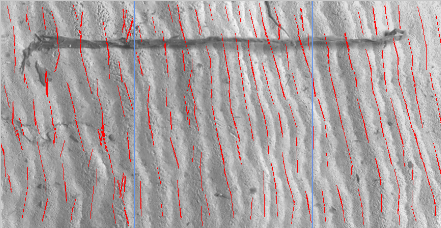
\includegraphics[width = 2.5in]{img/ManualUsuario/Cordillera}}
\subfloat{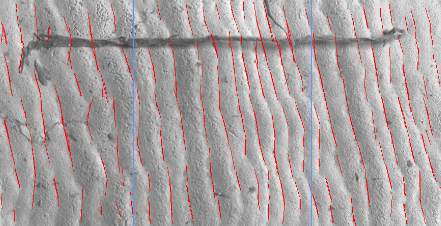
\includegraphics[width = 2.5in]{img/ManualUsuario/Valle}}
\caption[Opciones orientación de perikymata]{Opciones Vertical (izda.) y Vertical 2 (dcha.)}
\label{fig:PerikymataOrientation}
\end{figure}

Para terminar esta fase, comentaremos que también tenemos un botón \textit{Reset View} para volver a comenzar el proceso si los resultados no son los esperados. Este botón cargará la imagen recortada original.

\newpage
\subsection{Marcado de perikymata y exportación de datos}

Con la imagen ya filtrada pulsaremos el botón representado por un \textit{icono} de una línea. Pulsaremos y arrastraremos sobre la imagen pasando por las perikymata detectadas (color rojo) para que la aplicación pueda marcarlas posteriormente. También podemos ir pulsando sobre la imagen para que la línea se vaya creando. Si la línea excede los límites de la imagen, aparecerá un mensaje de error. El botón \textit{Clear Line} permite borrar la línea si no nos hemos equivocado.

Al pulsar el botón \textit{Auto-mark perikymata} se marcarán en verde las perikymata rojas por donde hemos pasado la línea (figura \ref{fig:img/ManualUsuario/FaseMarcado}). Es posible que algunos puntos verdes no sean verdaderamente una perikymata y otros puntos que se han quedado sin marcar sí; para ello disponemos en la esquina superior derecha de dos botones que nos permitirán añadir y quitar perikymata a la imagen. 

\imagenDos{img/ManualUsuario/FaseMarcado}{Marcado de perikymata}{1.02}

Una vez todo esté de nuestro gusto, pulsaremos el botón \textit{Export Data} y se guardará un fichero \textit{csv} en la carpeta del proyecto \textit{Perikymata\_Outputs}. Este archivo contendrá las perikymata marcadas, el decil en el que se encuentran, sus coordenadas en píxeles, y la distancia a la perikyma anterior.

\subsection{Otras funcionalidades}
En la parte superior de la ventana (figura \ref{fig:img/ManualUsuario/Menu}), tenemos tres menús con distintos botones, explicaremos los más relevantes.
\imagenDos{img/ManualUsuario/Menu}{Funcionalidades comunes}{0.35}

En el menú \textit{File} tenemos los siguientes botones:
\begin{itemize}
    \item \textit{New Proyect}: crea un nuevo proyecto en el que poder trabajar.
    \item \textit{Open Project}: permite abrir otros proyectos que tengamos.
    \item \textit{Save}: guarda el estado del proyecto.
    \item \textit{Close}: cierra la aplicación.
\end{itemize}

En el menú \textit{Configuration} tenemos:
\begin{itemize}
     \item \textit{Full Screen}: hace que la ventana de la aplicación se maximice. Es útil en etapas como la del filtrado y recuento de perikymata, pues permite ver mejor toda la interfaz.
      \item \textit{Set temporary folder}: para la unión de imágenes se necesita utilizar una carpeta sin rutas con espacios en blanco como carpeta temporal. Esta opción abre una ventana como la de la figura \ref{fig:img/ManualUsuario/CarpetaTemporal} para permitirnos seleccionar una carpeta temporal de nuestra elección. La aplicación mostrará un mensaje de error si se intenta seleccionar una carpeta con espacios en blanco en su ruta.
      
      \imagenDos{img/ManualUsuario/CarpetaTemporal}{Elección de carpeta temporal}{0.65}
\end{itemize}

En relación con este apartado, hay que explicar uno de los errores que se han encontrado al usar la aplicación en Linux. Puede darse la ocasión en que los botones de menú de la parte superior no respondan y que tampoco se pueda redimensionar la ventana. Salvo eso, la aplicación funciona con normalidad. Se desconoce el origen del error.


\subsection{Observaciones}

Sobre las imágenes a filtrar:\\
Las imágenes de fragmentos que se han proporcionado para este proyecto suelen venir incluidas en una carpeta. En ella encontramos imágenes con la leyenda que indica la medida y las mismas imágenes pero sin la leyenda. 

Para que las imágenes se puedan unir correctamente, es necesario que se escojan todas las imágenes sin leyenda menos una, para poder tomar la medida en la etapa correspondiente de la aplicación. Se recomienda que la imagen con la medida sea una de las esquinas, para interferir lo más mínimo con la operación de unión. Además, es labor del usuario que estas estén orientadas en el mismo sentido, de modo que las perikymata queden de forma vertical. Si al unir las imágenes obtenemos una imagen completamente negra, es posible que debamos eliminar de la lista alguna imagen muy similar a otra, porque esta puede comprometer la operación.

Sobre la aplicación en Linux y los scripts proporcionados:\\
Los usuarios de Windows pueden ver si funciona el servidor en una ventana de comandos, pero los usuarios de Linux no. Por eso en la carpeta \textit{PythonApp}, que contiene el servidor, se proporcionan los siguientes \textit{scripts} por si los usuarios encuentran dificultades para usar la aplicación por problemas del servidor:
\begin{itemize}
     \item \textit{StartServerLinux.sh}: enciende el servidor.
     \item \textit{StopServerLinux.sh}: detiene el proceso \textit{python3} que usa el servidor.
\end{itemize}

Para poder usarlos, habría que abrir una terminal dentro de la carpeta \textit{PythonApp} y escribir los siguientes comandos para cada \textit{script}. El primer comando solo es necesario la primera vez:\\
\centerline{\textit{\$ chmod +x script.sh}}
\centerline{\textit{\$ ./script.sh}}

Hay que comentar también, que los scripts están hechos para ejecutarse en una \textit{shell} de \textit{bash}, como la de Ubuntu, por ejemplo. Si se utiliza otra \textit{shell}, los usuarios pueden modificar los \textit{scripts} para adaptarlos.


\bibliographystyle{plain}
\bibliography{bibliografiaAnexos}

\end{document}
